\documentclass[a4paper,12pt]{article}

\usepackage{algpseudocode, amsfonts, amsmath, amssymb, amsthm, enumitem, fancyhdr, tikz}
\usepackage[plain]{algorithm}
\usepackage[margin=3.5cm]{geometry}
\usetikzlibrary{automata, positioning}
\allowdisplaybreaks
\pagestyle{fancy}

\renewcommand{\thesubsection}{\arabic{subsection}}
\newtheorem{theorem}{Theorem}
\newtheorem{lemma}[theorem]{Lemma}
\theoremstyle{remark}
\newtheorem{remark}{Remark}
\theoremstyle{definition}
\newtheorem{definition}{Definition}

\begin{document}

\section*{CS 4510-B Notes}


\subsection*{Introduction}

\subsubsection*{08/23/16}
\subsubsection*{08/25/16}
One of the most important developments in theoretical computer science is representing information as bits. \par
Intro to mathematics. There are many proofs of the fact that there are infinitely many prime numbers. \par
Rest of class spent working in groups on the first set of puzzles.
\subsubsection*{08/30/16}
We can visualize several levels of abstractions in which the levels from bottom to top are, in order, \emph{strings}, \emph{problems}, \emph{algorithms}, and \emph{complexity classes}. \par

\subsection*{Sets}
Consider a set of strings $S \subseteq \{ 0, 1 \}^*$. Given a string $x \in \{ 0, 1 \}^*$, how do we determine whether $x \in S$ or $x \notin S$? \par
\textbf{I. Finite Sets.} A finite set has a finite number of elements, and finite sets $A$, $B$ have the set operations $A \cup B$, $A \cap B$, and $A - B$. Example of a finite set: acceptable passwords of length 8 using the letters A-Z. \par
\textbf{II. Regular Sets.} The empty string is $\epsilon$. New operations: the concatenation operation is given by
\begin{align*}
    A \cdot B = \{ x_1 \cdots x_k y_1 \cdots y_l \mid x_1 \cdots x_k \in A, \; y_1 \cdots y_l \in B \}
\end{align*}
and the Kleene star is given by
\begin{align*}
    A^* = \bigcup_{i \in \mathbb{N}} A_i
\end{align*}
where
\begin{gather*}
    A_0 = \{ \epsilon \} \\
    A_1 = A \\
    A_{i + 1} = \{ st \mid s \in A_i, \; t \in A \} \; \forall i > 0.
\end{gather*} \par
Finite sets $\subseteq$ regular sets. The previous definition was very math-oriented. How is it defined from the perspective of computer science? \par
\textbf{DFA (deterministic finite automaton):} \par
Input: a string $x_1 \cdots x_n \in S$. The procedure is given by
\begin{algorithm}[H] {\begin{algorithmic}[1]
    \State $c \leftarrow 0$
    \Loop
        \State $z \leftarrow \text{current symbol}$
        \If {$z$ is null}
            \State answer is ---
        \EndIf
        \State $c \leftarrow \text{process}(z, c)$
    \EndLoop
    \State answer is ---
\end{algorithmic}} \end{algorithm}
$c$ is a \emph{state} in a finite set of states. In DFA diagrams, states are represented using circles, and transitions between states are represented using arrows labeled by symbols. A state represented by a circle concentric inside another is an \emph{accepting state}, which indicates that the string of symbols processed so far is part of the regular set. Here is an example of a diagram for a DFA which accepts strings of even length:
\begin{center}
    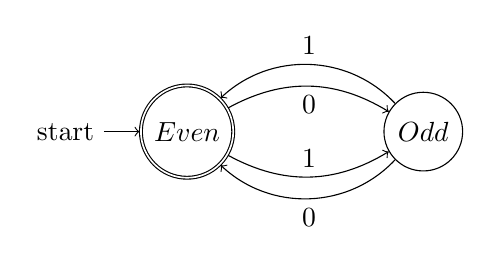
\begin{tikzpicture}[node distance=3cm, on grid, auto] 
        \node[state,initial,accepting] (even) {$Even$}; 
        \node[state](odd) [right=of even] {$Odd$};
        \path[->]
        (even) edge [bend left, swap] node {0} (odd)
            edge [bend right] node {1} (odd)
        (odd) edge [bend left=45] node {0} (even)
            edge [bend right=45, swap] node {1} (even);
    \end{tikzpicture}
\end{center}

\subsubsection*{09/06/16}
\subsection*{Strings and Languages}
Let $\Sigma$ denote an alphabet, e.g.
\begin{itemize}
    \item
        $\Sigma_1 = \{ 0, 1 \}$
    \item
        $\Sigma_2 = \{ a, b, c, \cdots, z \}$
\end{itemize}
Then a \emph{language} is a set of strings whose characters take values over $\Sigma$. Given the alphabet $\Sigma_1$, a state diagram for an example language is given below:
\begin{center}
    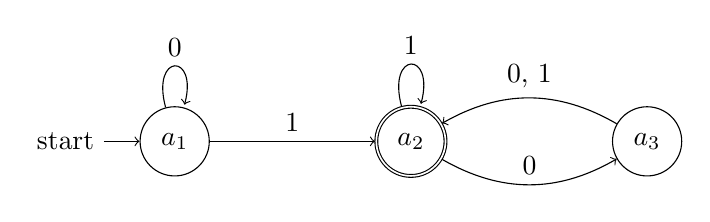
\begin{tikzpicture}[node distance=3cm, on grid, auto] 
        \node[state,initial] (a1) {$a_1$}; 
        \node[state,accepting](a2) [right=of a1] {$a_2$};
        \node[state](a3) [right=of a2] {$a_3$};
        \path[->]
        (a1) edge node {1} (a2)
            edge [loop above] node {0} (a1)
        (a2) edge [loop above] node {1} (a2)
            edge [bend right] node {0} (a3)
        (a3) edge [bend right, swap] node {0, 1} (a2);
    \end{tikzpicture}
\end{center}
Given the input $1101$, the actions taken are as follows:
\begin{itemize}
    \item
        Consume 1, go to state $a_2$,
    \item
        Consume 1, remain at state $a_2$,
    \item
        Consume 0, go to state $a_3$,
    \item
        Consume 1, go to state $a_2$.
\end{itemize}
\begin{definition}
    A \emph{DFA} is a 5-tuple $(Q, \Sigma, \delta, q_0, F)$ where
    \begin{itemize}
        \item
            $Q$ is a finite set of states,
        \item
            $\Sigma$ is a finite alphabet,
        \item
            $\delta : Q \times \Sigma \to Q$ is the \emph{transition function},
        \item
            $q_0 \in Q$ is the starting state, and
        \item
            $F \subseteq Q$ is the set of accepting states.
    \end{itemize}
\end{definition}
\textbf{Computation:}
\begin{definition}
    $M = (Q, \Sigma, \delta, q_0, F)$, $\omega = \omega_1 \omega_2 \cdots \omega_n, |\omega| = n$. $M$ will \emph{accept} $\omega$ if there is a sequence of states $r_0, r_1, \cdots, r_n$ in $Q$ such that
\begin{enumerate}
    \item
        $r_0 = q_0$,
    \item
        $\delta(r_i, \omega_{i + 1}) = r_{i + 1}, i \in [0, n - 1]$,
    \item
        $r_n \in F$.
\end{enumerate}
A language is called a \emph{regular language} if some finite automaton recognizes it. \par
\end{definition}
Designing DFA example: Given $\Sigma = \{ 0, 1 \}$, what is the DFA for the language $L(H) = \{ w \mid w \text{ has an odd \# of 1's}\}$?
\begin{center}
    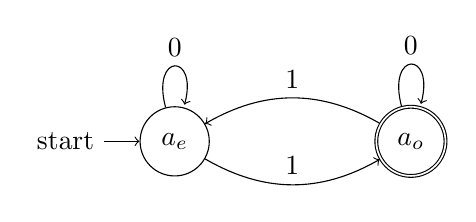
\begin{tikzpicture}[node distance=3cm, on grid, auto] 
        \node[state,initial] (ae) {$a_e$}; 
        \node[state,accepting](ao) [right=of ae] {$a_o$};
        \path[->]
        (ae) edge [loop above] node {0} (ae)
            edge [bend right] node {1} (ao)
        (ao) edge [loop above] node {0} (ao)
            edge [bend right, swap] node {1} (ae);
    \end{tikzpicture}
\end{center}
\textbf{Regular operations:}
\begin{itemize}
    \item
        Union: $A \cup B = \{ x \mid x \in A \text{ or } x \in B \}$
    \item
        Concatenation: $A \cdot B = \{ xy \mid x \in A \text{ and } y \in B \}$
    \item
        Star: $A^* = \{ x_1 x_2 \cdots x_n \mid k \geq 0, x_i \in A \}$
\end{itemize}
\textbf{NFA (nondeterministic finite automaton):} \par
Differences from DFAs:
\begin{itemize}
    \item
        Transitions output a set of states instead of a single state
    \item
        $\epsilon$-transitions, which may occur from a state without requiring an input
\end{itemize}
\begin{definition}
    An \emph{NFA} is a 5-tuple $(Q, \Sigma, \delta, q_0, F)$ where
    \begin{itemize}
        \item
            $Q$ is a finite set of states,
        \item
            $\Sigma$ is a finite alphabet,
        \item
            $\delta : Q \times (\Sigma \cup \{\epsilon\}) \to P(Q)$ is the transition function, where $P(Q)$ is the power set of $Q$,
        \item
            $q_0 \in Q$ is the \emph{starting state},
        \item
            $F \subseteq Q$ is the set of \emph{accepting states}.
    \end{itemize}
\end{definition}
\begin{theorem}
    Every NFA has an equivalent DFA.
\end{theorem}
\begin{proof}
    Let $N = (Q, \Sigma, \delta, q_0, F)$ be an NFA. If we let
    \begin{itemize}
        \item
            $Q' = P(Q)$,
        \item
            For $R \in Q'$ and $a \in \Sigma$,
            \begin{align*}
                \delta'(R, a) = \{ q \in Q \mid q \in E(\delta(r, a)) \text{ for some } r \in R \},
            \end{align*}
        \item
            $q_0' = E(\{ q_0 \})$,
        \item
            $F' = \{ R \in Q' \mid R \text{ contains an accepting state of } N \}$,
    \end{itemize}
    where $E(R) = \{ q \mid q \text{ can be reached from some $r \in R$ by taking $0$ or more $\epsilon$-transitions} \}$, then $(Q', \Sigma, \delta', q_0', F')$ is a DFA which accepts strings from the same language as $N$.
\end{proof}
When converting an NFA to a DFA, the trickiest part is evaluating the transition function $\delta'$ for every input. \par
An additional simplification may be made -- some states in $Q'$ may be unreachable if they are not starting states and have no outgoing transitions, so they may be removed.

\subsubsection*{09/08/16}
\emph{Crossing sequences} are an application of NFAs. These are sequences in which, given a partition of the possible states, the state at some point in the sequence becomes part of a different set. \par
An example of a non-regular language:
\begin{align*}
    L = \{ 0^n 1^m \mid n = m \geq 1 \}
\end{align*}
This is because $n$ and $m$ can get arbitrarily big. The pumping lemma can be used to prove that languages are not regular.

\subsubsection*{09/13/16}
\textbf{DFA, NFA, 2-way DFA, Regular Expressions:} \par
The $\$$ symbol is a convenient way to denote the end of an input. \par
In a \emph{2-way DFA}, you can either go either left or right in the input and read the symbol at that location. Such an input is called a \emph{2-way tape} and \emph{read-only}. Note that it must have a $\$$ symbol at both the beginning and the end. \par
The language $\$0^n 1^m\$$ is not regular. However, if you could write on the tape then it would be recognizable by some automaton. It would recognize it by alternately checking off $0$s from the beginning and $1$s from the end of the input. \par
\textbf{Turing:} \emph{write} new symbols, tape \emph{unlimited} \par
\textbf{Church's Thesis:} Turing machine is as powerful as calculating by hand

\subsubsection*{09/15/16}
It is easiest to represent a Turing machine by a table of states and symbols, and a table of instructions that tell the machine what to write at the current square, whether to move the tape head left or right, and what the next instruction should be. \par
A Turing machine can be designed to add numbers by adding bits in order, taking carries into account. The \textbf{copy} subroutine is crucial for multiplying numbers. \par
There is also a type of Turing machine with multiple \emph{tracks}, so that the tape head reads from and writes to the square in all tracks at once.

\subsubsection*{09/20/16}
Denote $M_x(y)$ as the answer machine $M_x$ on input $y$. Then $M_x(y)$ is doable by a Turing machine. \par
A \emph{universal Turing machine} is a Turing machine that can simulate an arbitrary Turing machine on an arbitrary input. \par
\textbf{Halting problem:} Given $x$, $y$, determine whether $M_x(y)$ is defined.
\begin{theorem}
    The halting problem is not computable:
    \begin{align*}
        H(x, y) = \begin{cases}
            1 \textnormal{ if } M_x(y) \textnormal{ answers} \\
            0 \textnormal{ if } M_x(y) \textnormal{ never stops}
        \end{cases}.
    \end{align*}
    \begin{proof}
        Assume for the purpose of contradiction that $H(x, y)$ is computable. Let $f(x) = M_n(x)$ and
        \begin{align*}
            f(x) = 1 + \sum_{y = 0}^x H(x, y) \cdot M_x(y).
        \end{align*}
        Then
        \begin{gather*}
            f(n) = 1 + \sum_{y = 0}^n H(n, y) \cdot M_n(y) \\
            \Rightarrow M_n(n) = f(n) = 1 + \sum_{y = 0}^n M_n(y) \geq 1 + M_n(n),
        \end{gather*}
        a contradiction.
    \end{proof}
\end{theorem}
\subsubsection*{09/22/16}
More generally, Cantor's \emph{diagonalization} argument can be used to show that the set of all languages is uncountable while the set of all Turing machines is countable; hence, other languages are also not Turing-decidable. In particular, the halting problem has its own diagonalization argument which shows its uncomputability by contradiction. The class is referred to the book for more details.
\subsubsection*{09/27/16}
We can show that other problems are not computable by \emph{reducing} them to the halting problem. (Joke about mathematician reducing to a problem already solved) \par
An \emph{undecidable} decision problem is one for which no algorithm exists. \textbf{Rice's theorem:} Any nontrivial property about the language recognized by a Turing machine is undecidable.

Diversion to ``natural problems.'' \par
Number theory: the Diophantine equation $x^2 = 2y^2$ has no integer solutions, while $x^2 + 2 = y^3$ has a solution $x = 5, y = 3$. Another example: $x^3 + y^3 = z^3$. Summarized in \emph{Hilbert's Tenth Problem}. It turns out this is NOT computable, but we can use approximations such as having $2^x$ terms.

\subsubsection*{09/29/16}
Variations of Turing machines:
\begin{enumerate}
    \item
        2-tape machine
    \item
        Multi-tape machine
    \item
        Read-only input
    \item
        One-way tape
    \item
        Big alphabet (each letter can be represented as $01$-string)
    \item
        Turing machine that accepts $0^n 1^n$ takes $n^2$ steps
\end{enumerate}

\subsubsection*{10/04/16}
\textbf{Practice midterm review:}
\begin{enumerate}
    \item
        \begin{enumerate}
            \item
                $A \setminus B = \{ x \mid x \in A \text{ and } x \notin B \}$
            \item
                $A \cap B = \{ x \mid x \in A \text { and } x \in B \}$
            \item
                $A \cdot B = \{ xy \mid x \in A \text { and } y \in B \}$
        \end{enumerate}

    \item
        Let $A$ be finite, $B$ non-regular. Then $A \setminus B$ is finite, so it is regular. However, $B \setminus A$ is still non-regular.

    \item
        We know that $f(p) = M_p(p)$ is not computable from the proof of contradiction that the halting problem is not computable. Another way to denote $f(p)$ is by saying ``use program $p$ to simulate $M_x(x)$.''

    \item
        Just add one or more dummy states to $M_x(y)$ that both is reached from and reaches other states by $\epsilon$-transitions. For example, add another state reachable from the final state of $M_x(y)$ by an $\epsilon$-transition.
\end{enumerate}

\subsubsection*{10/13/16}
Time and \emph{space} considerations in Turing machines:
\begin{definition}
    A language $L \in \text{DSPACE}(f(n))$ if there exists a Turing machine recognizing $L$ that uses at most $O(f(n))$ space on inputs of length $n$.
\end{definition}
Note: usage of memory space can be achieved in a Turing machine by writing to empty locations on the tape. \par
For example, $\{ 0^n 1^n \mid n \geq 1 \} \in \text{DSPACE}(\log(n))$ because we can keep counters for the number of $0$'s and $1$'s, which each use $\log(n)$ bits. \par
We also have the class $\text{NSPACE}(f(n))$, which is like $\text{DSPACE}(f(n))$ but for nondeterministic Turing machines. Any decision problem decided by a nondeterministic Turing machine is reducible to graph reachability, where the graph is constructed by having states correspond to vertices and transitions correspond to edges.

\subsubsection*{10/18/16}
We have the following powerful theorems:
\begin{theorem}[Savitch]
    $\text{NSPACE}(\log n) \subseteq \text{DSPACE}(\log^2 n)$.
\end{theorem}
\begin{theorem}
    $A \in \text{NSPACE}(\log n) \Rightarrow \overline{A} \in \text{NSPACE}(\log n)$.
\end{theorem}
\begin{theorem}
    $\text{DSPACE}(\log n) \subsetneq \text{DSPACE}(\log^2 n)$.
\end{theorem}
$A$ can be represented as a set of paths in a graph $G$:
\begin{align*}
    A = \{ (G, s, f) \mid s \rightarrow \cdots \rightarrow f \}
\end{align*}
\textit{Sketch of proof of Savitch's theorem:} \par
Let $[x, y, k]$ be the set of all paths from $x$ to $y$ of length $\leq k$. Then our approach is to recursively compute $\{ [x, z, k/2], [z, y, k/2] \}$ for all $z$ until the path length becomes $1$. \par
Now apply this to $[s, f, n]$ to see if a path exists from $s$ to $f$. \par
Alternatively, count the number of paths in the \emph{reachability set} $R_k$ from $s$ to $x$. The set might be too big, so a workaround is to formulate it in terms of a \emph{generator}: guess the sequence $\rightarrow R_k$, and generate for $v = 1, \cdots, n$. \par
This problem was open for 30-40 years, but was solved simultaneously by two different people.

\subsubsection*{10/20/16}
Overview of some projects: \par
Presburger arithmetic is a language with the alphabet $\{0, 1\}$ and the binary addition operation $+$. Part of the theorem states that
\begin{gather*}
    \forall x, \exists y \text{ s.t. } y > x, \\
    y > x \Leftarrow \exists z \text{ s.t. } y = x + z \land z \neq 0
\end{gather*} \par
Probabilistic finite state machines can accept non-regular languages such as $0^n 1^n$. \par
One ramification of Post's theorem is that if $A$ and $\overline{A}$ are both computable, then there exists an algorithm for $A$. \par
The minimum description length of data is the fewest number of bits to which the data can be compressed. \par
Ladner's theorem states that if $P \neq NP$, then there exists some kind of ``middle ground.'' \par
A boolean function is a function $f : \{ 0, 1 \}^n \to \{ 0, 1 \}$. Any boolean function can be computed by a circuit.

\subsubsection*{10/25/16}
Initial reasoning for the Card Trick puzzle: There are only $4! = 24$ different arrangements of $4$ cards. The other insight is that Alice can choose which of the five cards to hand back to the audience member. By the pigeonhole principle, at least two cards must share the same suit. \par
More general statements of theorems:
\setcounter{theorem}{2}
\begin{theorem}
    $\text{NSPACE}(f(n)) \subseteq \text{DSPACE}(f^2(n))$.
\end{theorem}
\begin{theorem}
    $\text{NSPACE}(f(n)) = \text{co\text{-}NSPACE}(f(n))$.
\end{theorem}
\begin{theorem}
    $\text{DSPACE}(g(n)) \subsetneq \text{DSPACE}(f(n))$, $\frac{f(n)}{g(n)} \to \infty$.
\end{theorem}
\noindent Continuation of proof sketch of Savitch's theorem: $R_k$ has generator $s_0, s_1, \cdots, s_m$. We can construct a generator for $R_k$ if we know $|R_k|$.
\begin{algorithm}[H] {\begin{algorithmic}[1]
    \For {$r = 1, \cdots, n$}
        \If {there is a path of length $\leq k$ from $s \rightarrow r$}
            \State output($v$)
        \EndIf
    \EndFor
\end{algorithmic}} \end{algorithm}
We have $R_0$, and for every $|R_{k - 1}|$, we can deduce $|R_k|$ as follows:
\begin{algorithm}[H] {\begin{algorithmic}[1]
    \For {$v = 1, \cdots, n$}
        \If {there is a path from $w \rightarrow r$ for some $w \in R_{k - 1}$}
            \State $|R_k|{++}$
        \EndIf
    \EndFor
    \State \Return $|R_k|$
\end{algorithmic}} \end{algorithm}

\subsubsection*{10/27/16}
\textbf{Time complexity:}
of a TM is just the number of steps before it halts. Remarkable thing about memory is that it can be reused, but the same cannot be said about time. \par
$\text{NTIME}(t(n))$ and $\text{DTIME}(t(n))$ are the classes of languages that can be accepted by a nondeterminstic and a deterministic TM respectively in $O(t(n))$ time. \par
Our previous three theorems have no known analogues for time complexity (they are unsolved problems). \par
\textbf{Simulation:} A TM $M$ uses space $S$ and time $T$, and $U$ simulates $M$ in space $O(S)$. Can $U$ simulate $M$ in time $O(T)$? Another unsolved problem. We know that the answer is yes for $O(T^2)$ and for $O(T \log T)$.

\subsubsection*{11/01/16}
\textbf{$\text{P} \overset{?}{=} \text{NP}$:}
\begin{align*}
    \text{P} \triangleq \bigcup_{k \geq 1} \text{DTIME}(n^k)
\end{align*}
(In other words, $S$ is in $\text{P}$ if $\exists$ TM that accepts $S$ and runs in time $O(n^k)$.)
\begin{align*}
    \text{NP} \triangleq \bigcup_{k \geq 1} \text{NTIME}(n^k)
\end{align*}
Conjectures:
\begin{enumerate}
    \item
        $\text{P} \neq \text{NP}$.
    \item
        $\text{NP}$ is really hard: $\exists S \in \text{NP}$ that takes $2^n$ time on input of size $n$.
\end{enumerate}
$\text{NP}$ means ``easy to check.'' Given a solution to $S$, it can be verified in $O(n^k)$ time. If $\text{P} = \text{NP}$, then guessing and checking property is in $\text{DTIME}(n^{k^1})$. \par
Modern cryptography depends on the assumption that $\text{P} \neq \text{NP}$. \par
\textbf{Reduction}: $A \leq_{\text{poly}} B$ if there is a function $f(x)$ that computes, in poly-time,
\begin{align*}
    \forall x, x \in A \Leftrightarrow f(x) \in B
\end{align*}
\begin{theorem}
    $A \leq_{\textnormal{poly}} B$ if $B \in \text{P} \Rightarrow A \in \text{P}$.
\end{theorem}
$\text{NP} \overset{?}{=} \text{co-NP}$ \par
If $S \in \text{NP}$, we say that $S$ is \emph{complete} (NP-complete) if for all $T \in \text{NP}$, $T \leq_{\text{poly}} S$.

\subsubsection*{11/08/16}
The biggest theorem, \textbf{Cook's Theorem} (1971): \par
\noindent If a problem $S$ is NP-complete and can be solved in polynomial time, then any NP-complete problem can. \par
Fact: $S \leq_{\text{poly}} T$ if $T \in NP$. \par
\textbf{SAT}: given boolean variables $x_1, x_2, \cdots, x_n$ and clauses $\mathcal{C}_1, \mathcal{C}_2, \cdots, \mathcal{C}_m$ which are disjunctions of the boolean variables or their complements, we want to see if
\begin{align*}
    \mathcal{C}_1 \land \mathcal{C}_2 \land \cdots \land \mathcal{C}_m
\end{align*}
is satisfiable. Example: Sudoku is in NP because solutions can be verified in polynomial time, but is also NP-complete. \par
A $k$-clause is a disjunction of $k$ boolean variables or their complements. \par
Any problem $M$ in NP is reducible to SAT. This is shown using a \emph{tableau} for $M$ on input $w$, an $n^k \times n^k$ table whose rows are the configurations of a branch of the computation of $M$ on $w$. By checking entries, we can simulate satisfiability of parts of the expression separately. More can be found under the section ``The Cook-Levin Theorem'' in section 7.3 of the textbook.

\subsubsection*{11/10/16}
Back to $\text{P} = \text{NP}$: $\text{P} \subseteq \text{NP}$ \par
Fact: $\text{NTIME}(n^k) \subseteq \text{DTIME}(n^{k^1}) \Rightarrow \text{P} = \text{NP}$.
\begin{theorem}[Cook]
    $\text{SAT}$ is NP-complete.
\end{theorem}
\begin{theorem}[Karp]
    (Shows that 21 different decision problems are NP-complete)
\end{theorem}
SAT and $\text{SAT}_i$:
\begin{gather*}
    y \in T \Leftrightarrow f(y) \in \text{SAT} \\
    y \in T \Leftrightarrow g(y) \in \text{SAT}_i \\
    g(y) = \begin{cases}
        y \text{ is a bad input } \rightarrow \text{ ask a better question } \rightarrow f(z), z = y \land \{t\} \\
        y \text{ is not a bad input } \rightarrow f(y)
    \end{cases}
\end{gather*}
We use the \emph{padding} technique above: given a set of $m$ clauses, if a new clause $\{t\}$ is added, then the original set of clauses is satisfiable if and only if the new set of clauses is. \par
SAT has more of a flavor of formal logic. Karp was more of an operations research (ISYE to us) person, and the 21 problems he studied are highly practical.

\textbf{Practice Midterm 2 Review:}
\begin{enumerate}
    \item
        \begin{gather*}
            \text{P} = \bigcup_{k \geq 1} \text{DTIME}(n^k) \\
            \text{NP} = \bigcup_{k \geq 1} \text{NTIME}(n^k) \\
            \text{L} = \bigcup_{k \geq 1} \text{DSPACE}(\log n) \\
            \text{NL} = \bigcup_{k \geq 1} \text{NSPACE}(\log n)
        \end{gather*}
    \item
        Cook's theorem: SAT is NP-complete \\
        Savitch's theorem: $\text{NSPACE}(f(n)) \subseteq \text{DSPACE}\left( f(n)^2 \right)$ \\
        Immerman's theorem: If a language $A$ is in NSPACE, then so is its complement $\overline{A}$.
    \item
        Consider the set of expressions
        \begin{align*}
            (t \lor x \lor y \lor z) \land (\overline{t} \lor u \lor w)
        \end{align*}
        for $t = 0, 1$. If $x \lor y \lor z = 1$, then the expression in which $t = 0$ is satisfiable. If $u \lor w = 1$, then the expression in which $t = 1$ is satisfiable. If both are $1$, then both expressions are satisfiable, and if neither is $1$, then neither expression is satisfiable. Thus, in all cases, $A$ is equivalent to some expression of this form. \par
        When applied in general, this rule/technique is called a \emph{cut} or a \emph{resolution}.
    \item
        $T$ consists of $01$-strings of length $m$ in $S$ followed by $m^2$ $a$'s, so the length of the input is $n = m + m^2$, and $O(n) = O(m^2)$. Furthermore, it is given that the first part takes $O(m^2)$ time to decide, and the second part does as well since it is a constant string. Thus, the language takes $O(m^2) = O(n)$ time to compute.
\end{enumerate}
\end{document}
